\begin{figure}[t]
\centering       
    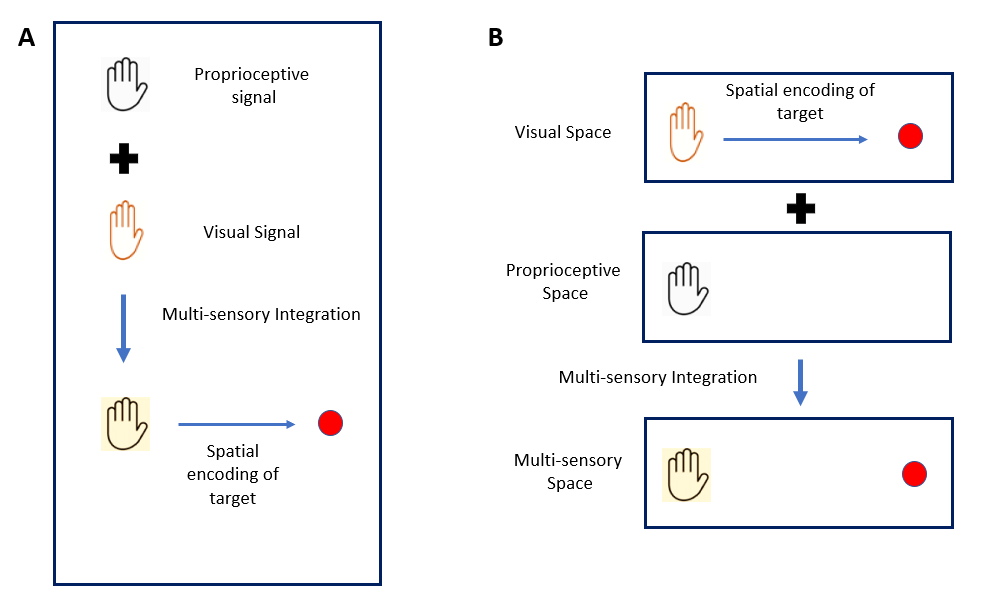
\includegraphics[width=\textwidth, keepaspectratio]{Images/ms_mechanisms.png}
    \caption{Two hypothesis regarding spatial encoding of the reach target. In A), the filled hand denotes the hand position inferred from the multi-sensory integration of visual and proprioceptive uni-sensory signals. The target's spatial location is encoded relative to this inferred hand position. In B) The target's spatial location is encoded relative to the visual signal in the visual space. The visual space is then integrated with the proprioceptive space to construct a multi-sensory representation of body-schema and surrounding peri-personal space.}
    \label{fig:ms-mechanisms}
\end{figure}